\documentclass[12pt, a4paper]{article}
\usepackage[utf8]{inputenc}
\usepackage[T1]{fontenc}
\usepackage[brazil]{babel}
\usepackage{graphicx}
\usepackage{hyperref}
\usepackage{geometry}
\usepackage{xcolor}
\usepackage{float}
\usepackage{tabularx}
\usepackage{booktabs}
\usepackage{listings}

\geometry{top=2.5cm, bottom=2.5cm, left=2.5cm, right=2.5cm}

\graphicspath{{resultados/}}

\title{Relatório Trabalho 3 \\ \large Sistema de busca e classificação de animais de estimação}
\author{Nome: Letícia Barbosa Neves \\ nUSP: 14588659}
\date{Semestre: 2026/1 \\ Disciplina: SCC0251 (Processamento de Imagens)}

\begin{document}

\maketitle

\section*{1. Introdução}
Este trabalho construiu um sistema de \textbf{classificação} e \textbf{busca por similaridade} sobre uma base de 367 fotos de 42 pets diferentes. Foram selecionados 5 descritores de imagem, extraídos para todas as imagens da base e depois avaliados isoladamente e em combinações, tanto para classificar a foto (identificar de qual pet é) quanto para recuperar fotos visualmente parecidas dada uma consulta.

\subsection*{Organização do Código}
\begin{table}[H]
\centering
\begin{tabularx}{\textwidth}{l X}
\toprule
\textbf{Arquivo / Pasta} & \textbf{Conteúdo} \\
\midrule
\texttt{codigos/descritores.py} & 5 extratores (HSV, HOG, LBP, ORB, Gabor) \\
\texttt{codigos/extrai\_features.py} & Pipeline de extração — salva todos os descritores em \texttt{.npy} \\
\texttt{codigos/classificacao.py} & Split 80/10/10 + Random Forest + matriz de confusão \\
\texttt{codigos/busca.py} & Busca por distância euclidiana + métrica P@k \\
\texttt{codigos/bovw.py} & KMeans sobre ORB $\to$ histograma de visual words \\
\texttt{codigos/visualizacao.py} & UMAP + t-SNE da BoVW \\
\texttt{features/} & Vetores extraídos (\texttt{.npy} / \texttt{.pkl}) \\
\texttt{resultados/} & Tabelas e figuras geradas \\
\bottomrule
\end{tabularx}
\end{table}

\subsection*{Instalação de dependências e inicialização}
Para instalar as bibliotecas necessárias:
\begin{lstlisting}[language=bash]
pip install numpy matplotlib imageio scikit-image scikit-learn umap-learn
\end{lstlisting}

Para executar o pipeline completo, no diretório do trabalho:
\begin{lstlisting}[language=bash]
python codigos/extrai_features.py
python codigos/classificacao.py
python codigos/busca.py
python codigos/bovw.py
python codigos/visualizacao.py
\end{lstlisting}

\newpage
\section*{2. Base de dados}
\begin{itemize}
    \item \textbf{367 imagens} em formato $256\times256$ RGB, distribuídas em \textbf{42 classes} (pets).
    \item Distribuição muito desbalanceada: classes vão de \textbf{1 a 20 imagens} por pet (kefka e hamtaro têm 20; vários pets têm apenas 1 ou 3 fotos).
    \item \textbf{5 classes têm apenas 1 imagem} (todos os \texttt{de\_bruno\_*}) --- excluídas da classificação conforme a regra do enunciado (``pets com menos de 3 fotos não entram''). Total efetivo para classificação: \textbf{362 imagens / 38 classes}.
\end{itemize}

\section*{3. Descritores escolhidos}
Foram selecionados 5 descritores cobrindo aspectos complementares da imagem: \textbf{cor} (HSV), \textbf{forma} (HOG), \textbf{textura local} (LBP), \textbf{pontos-chave} (ORB) e \textbf{textura estatística} (Gabor). A ideia foi escolher descritores que respondem a perguntas diferentes sobre o pet (``de que cor é?'', ``qual o contorno?'', ``qual o padrão do pelo?'', ``tem pontos marcantes?'', ``que escalas/orientações de padrão aparecem?''), pois para a tarefa de identificar um pet nenhuma característica isolada deveria ser suficiente.

Para cada descritor abaixo, apresentamos: a \textbf{justificativa da escolha}, a \textbf{semântica} capturada, a \textbf{hipótese} sobre as duas tarefas, o \textbf{resultado observado} e uma análise se a hipótese foi confirmada.

% --- HSV ---
\subsection*{3.1 Histograma HSV --- cor}

\textbf{Justificativa da escolha:} escolhemos HSV porque a primeira coisa que diferencia pets visualmente é a \textbf{cor do pelo}. HSV separa matiz (H) de brilho (V), o que é mais robusto a variação de iluminação do que histograma RGB simples --- duas fotos do mesmo pet em luzes diferentes têm cores RGB diferentes mas matiz parecida.

\textbf{Semântica capturada:} distribuição global de cor (quanto há de cada matiz, saturação e brilho), ignorando posição espacial.

\textbf{Implementação:} \texttt{color.rgb2hsv} (mesmo import do notebook \texttt{Aula17} da professora) + \texttt{np.histogram} em cada canal. Dimensão final: 96 ($3$ canais $\times$ $32$ bins, normalizado L1).

\textbf{Hipótese:}
\begin{itemize}
    \item \textbf{Classificação:} deve ser o descritor mais forte isoladamente, porque muitos pets têm cor de pelo característica.
    \item \textbf{Busca:} deve recuperar pets de cor parecida com a consulta, mesmo quando não acertar o pet exato.
\end{itemize}

\textbf{Resultado observado:} classificação acc $= 29.8\%$ (top-3 $= 48.9\%$), busca P@1 $= 25.1\%$. \textbf{Foi o melhor descritor isolado nas duas tarefas.}

\textbf{Confirmou a hipótese?} Sim. A matriz de confusão mostra confusões concentradas em pets de cores próximas; nos rankings de busca, vizinhos errados são tipicamente pets da mesma faixa cromática (branco fofo, caramelo, preto).

\begin{figure}[H]
    \centering
    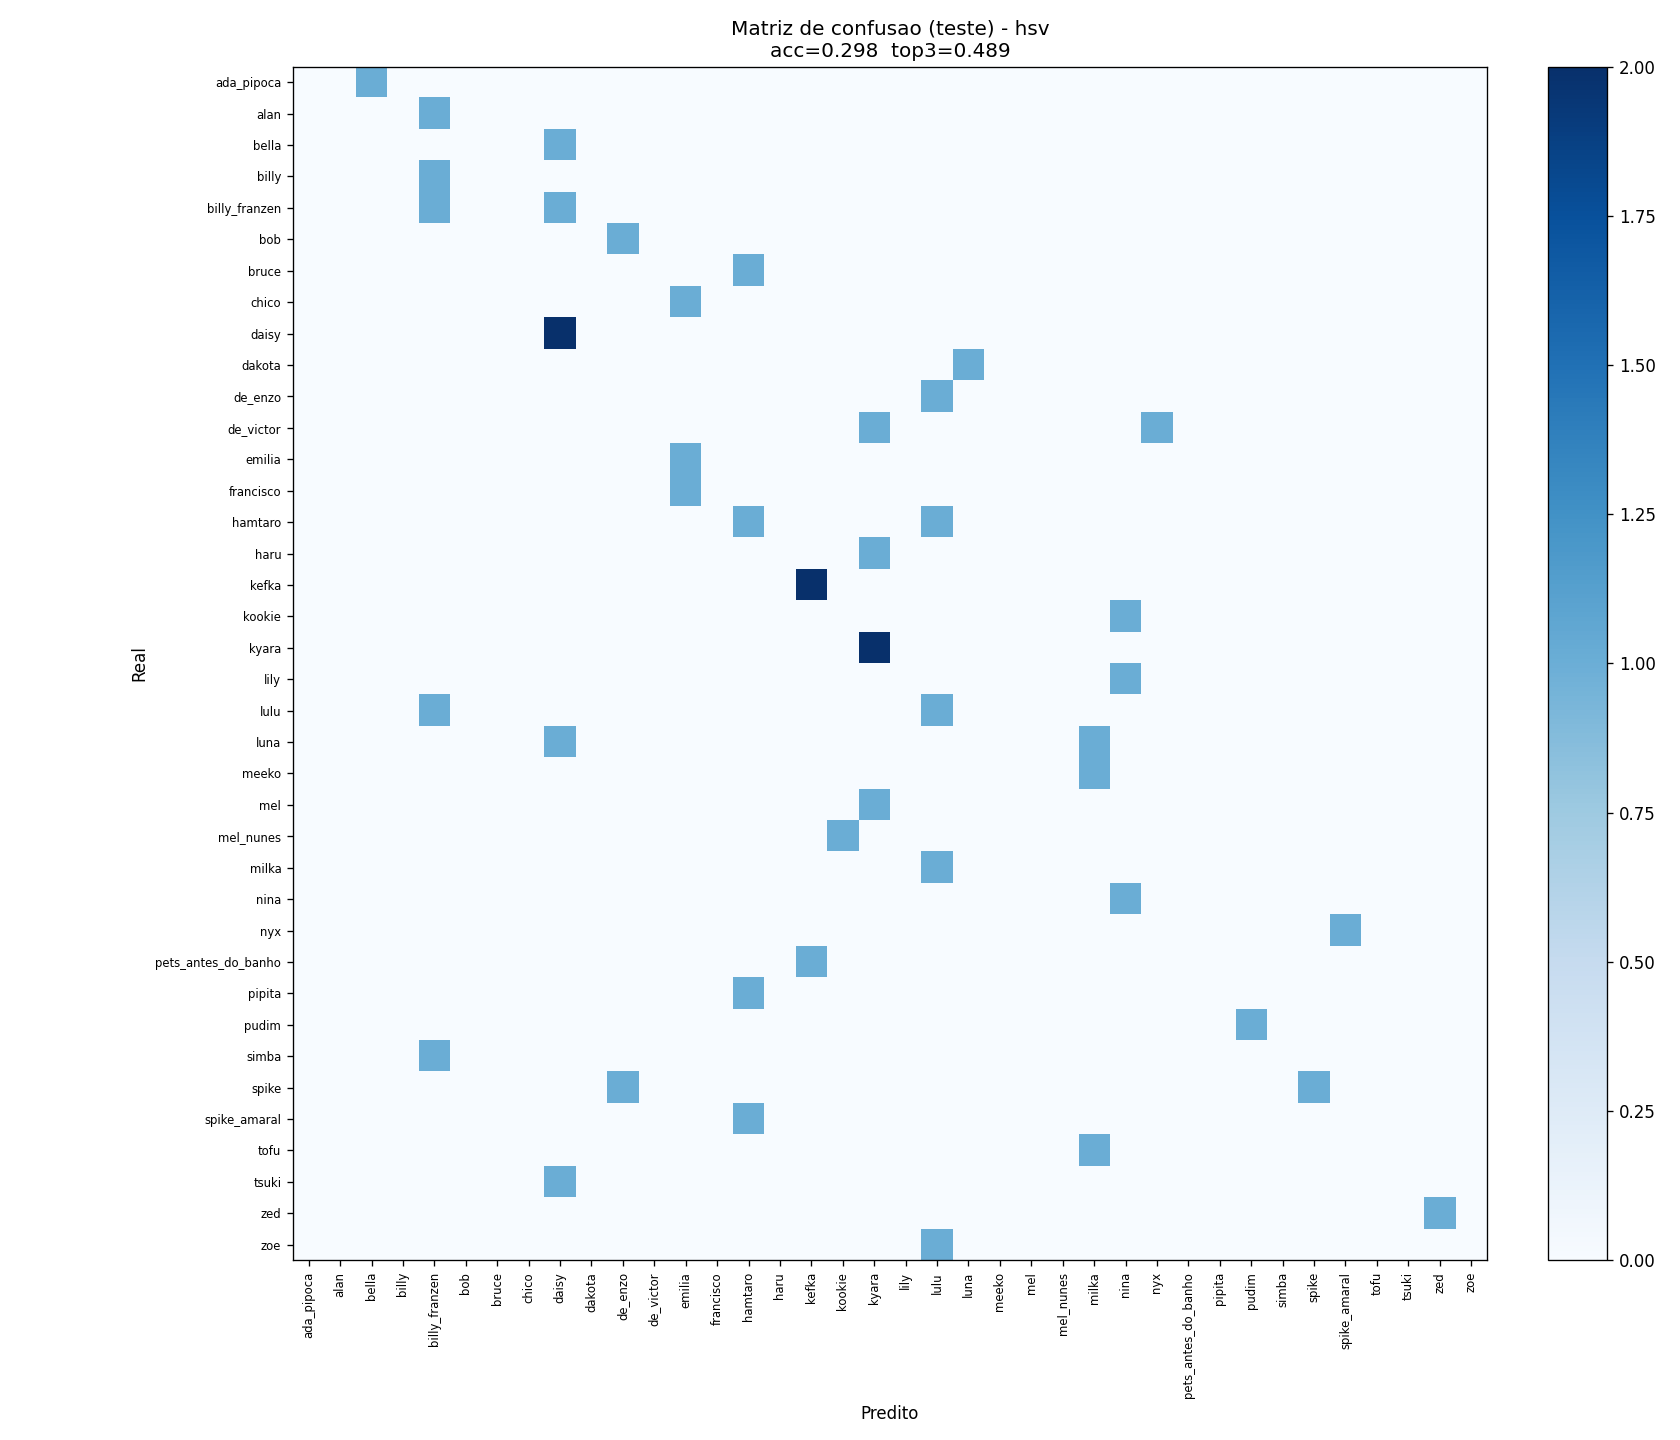
\includegraphics[width=0.75\textwidth]{classificacao_matriz_hsv.png}
    \caption{Matriz de confusão --- HSV isolado.}
\end{figure}

% --- HOG ---
\newpage
\subsection*{3.2 HOG --- forma / gradientes}

\textbf{Justificativa da escolha:} HOG foi escolhido para capturar a \textbf{silhueta} do pet --- descritor canônico para ``forma'' em visão computacional clássica e exatamente o tipo de descritor que a aula de segmentação cobriu. A hipótese era que pets com proporção corporal distinta (orelha em pé vs caída, focinho curto vs longo) teriam padrões de gradiente característicos.

\textbf{Semântica capturada:} histograma local de orientações de gradiente em uma grade sobre a imagem. Resume o padrão de bordas e contornos.

\textbf{Implementação:} \texttt{skimage.feature.hog} com \texttt{pixels\_per\_cell=(16,16)}, \texttt{cells\_per\_block=(2,2)}, 9 orientações. Dimensão final: \textbf{8100} (muito alta).

\textbf{Hipótese:}
\begin{itemize}
    \item \textbf{Classificação:} incerto. HOG é bom em domínios com pose padronizada (detector de pedestres clássico), mas pets aparecem em poses muito livres. Além disso, 8100 features para $\sim$290 amostras de treino é uma receita para overfitting.
    \item \textbf{Busca:} provavelmente fraco --- a alta dimensionalidade tende a dominar a distância euclidiana quando concatenada com outros descritores.
\end{itemize}

\textbf{Resultado observado:} classificação acc $= 12.8\%$ (pior individual), busca P@1 $= 9.4\%$ (pior individual). Em combinações com HSV, atrapalha em vez de ajudar (hsv+hog cai para P@1 $= 11.0\%$ vs HSV puro $25.1\%$).

\textbf{Confirmou a hipótese?} Sim, infelizmente. A matriz de confusão está muito esparsa e sem padrão claro na diagonal. \textbf{Lição metodológica:} para usar HOG numa base pequena seria essencial aplicar PCA antes (reduzir 8100 $\to$ $\sim$100 dims).

\begin{figure}[H]
    \centering
    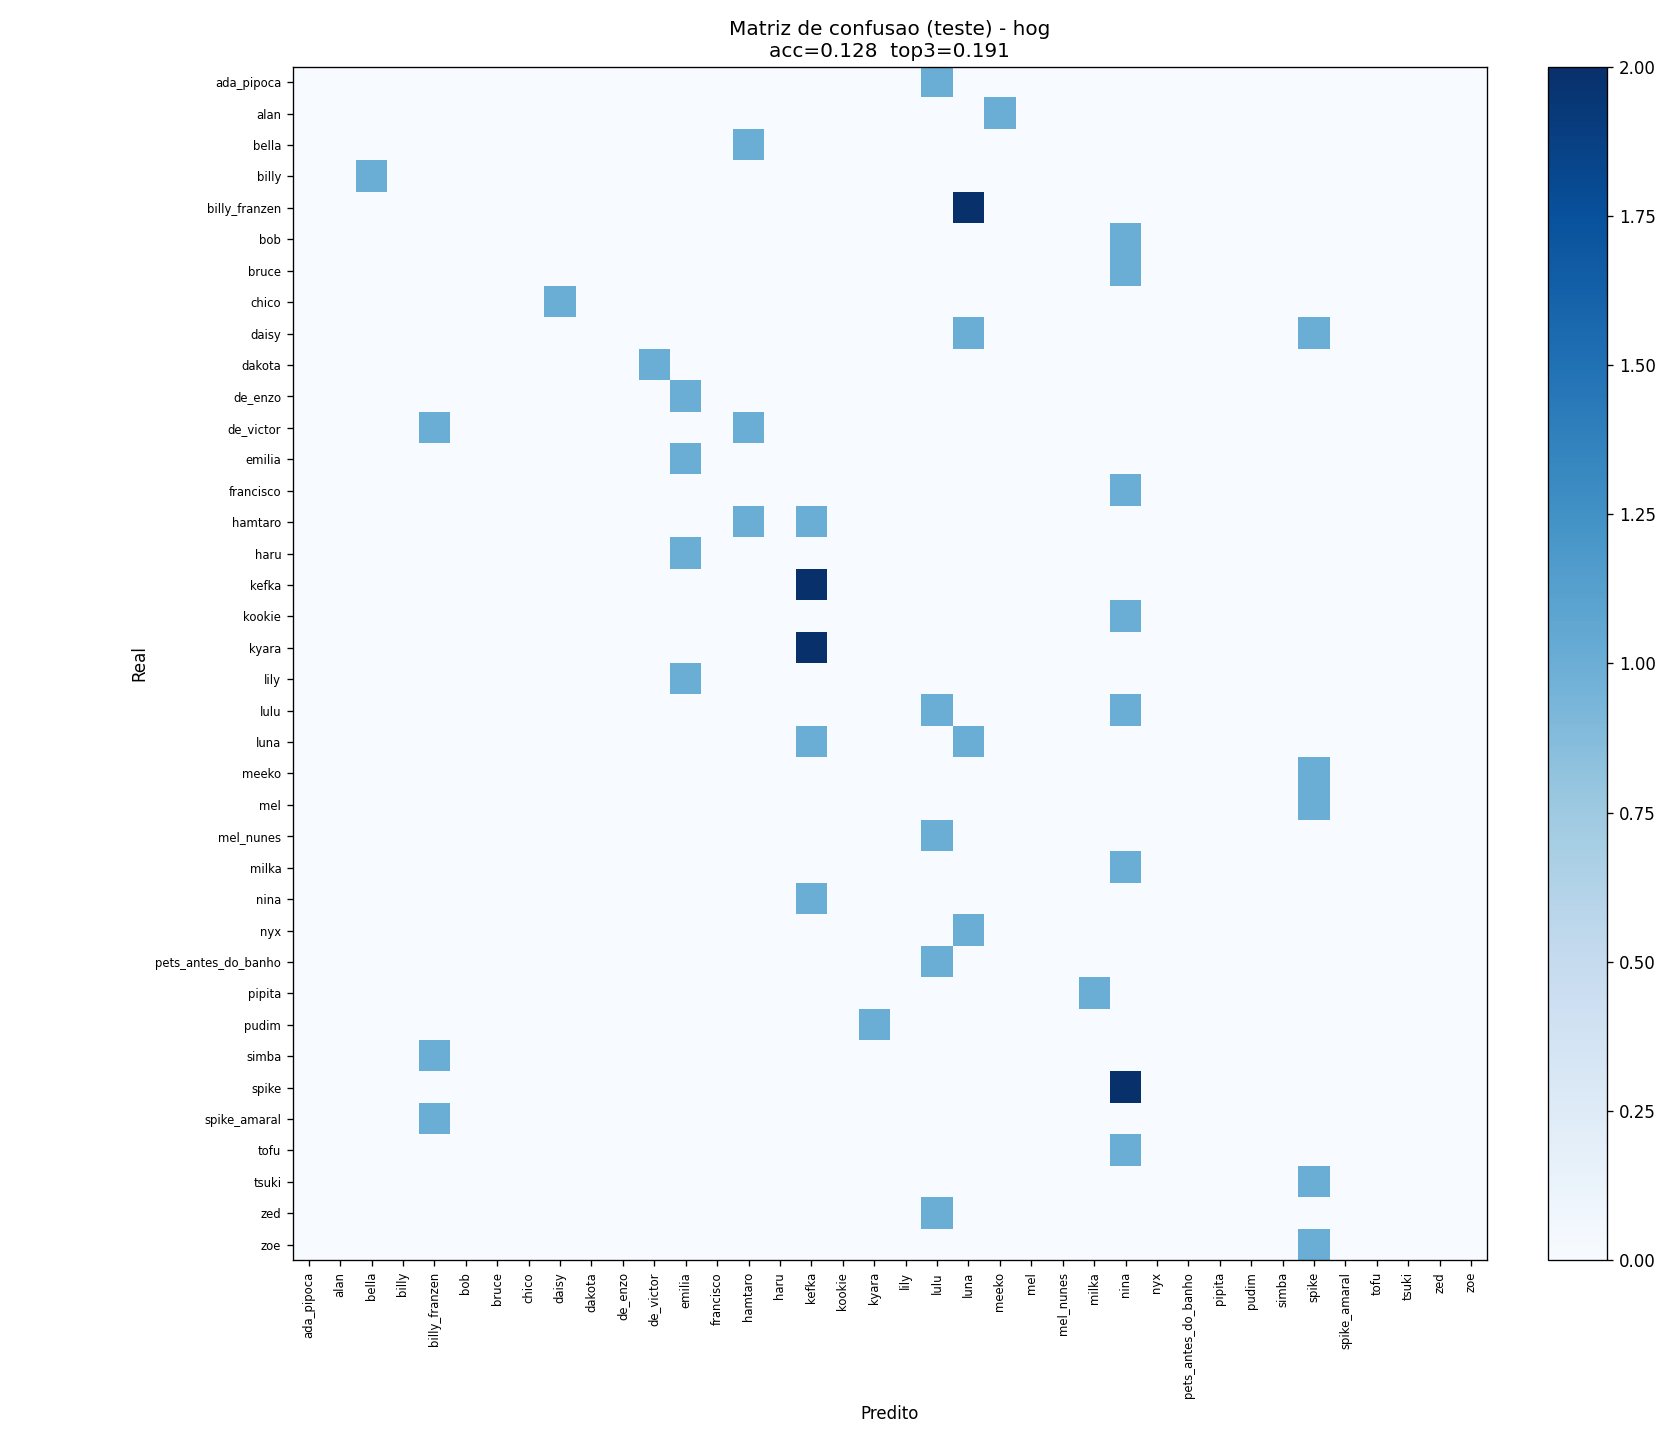
\includegraphics[width=0.75\textwidth]{classificacao_matriz_hog.png}
    \caption{Matriz de confusão --- HOG isolado.}
\end{figure}

% --- LBP ---
\newpage
\subsection*{3.3 LBP uniforme --- textura local}

\textbf{Justificativa da escolha:} LBP foi escolhido como um descritor de \textbf{textura barato e robusto a iluminação}. Comparado ao Gabor, é muito mais leve (10 features vs 32) e captura padrão local de microestrutura --- útil para diferenciar pelo curto vs longo, liso vs rajado. Também é descritor usado pela professora na aula de segmentação.

\textbf{Semântica capturada:} padrão binário do pixel central comparado aos 8 vizinhos. O histograma resume com que frequência cada padrão de textura local ocorre na imagem.

\textbf{Implementação:} \texttt{skimage.feature.local\_binary\_pattern} com \texttt{method='uniform'}, P=8, R=1. Dimensão final: 10.

\textbf{Hipótese:}
\begin{itemize}
    \item \textbf{Classificação:} descritor leve mas modesto. Não se espera que discrimine pets de pelo parecido (dois gatos pretos têm LBP parecido), mas pode ajudar como complemento à cor.
    \item \textbf{Busca:} provavelmente fraco sozinho, mas barato o suficiente para estar sempre na combinação.
\end{itemize}

\textbf{Resultado observado:} classificação acc $= 12.8\%$, busca P@1 $= 15.5\%$. Combinado com HSV (\texttt{hsv+lbp}) melhora ligeiramente a busca para P@1 $= 27.3\%$ (acima do HSV puro).

\textbf{Confirmou a hipótese?} Sim. Sozinho é modesto, mas faz seu papel como complemento --- a matriz mostra concentrações de erros em pets com texturas similares de pelo, exatamente como esperado.

\begin{figure}[H]
    \centering
    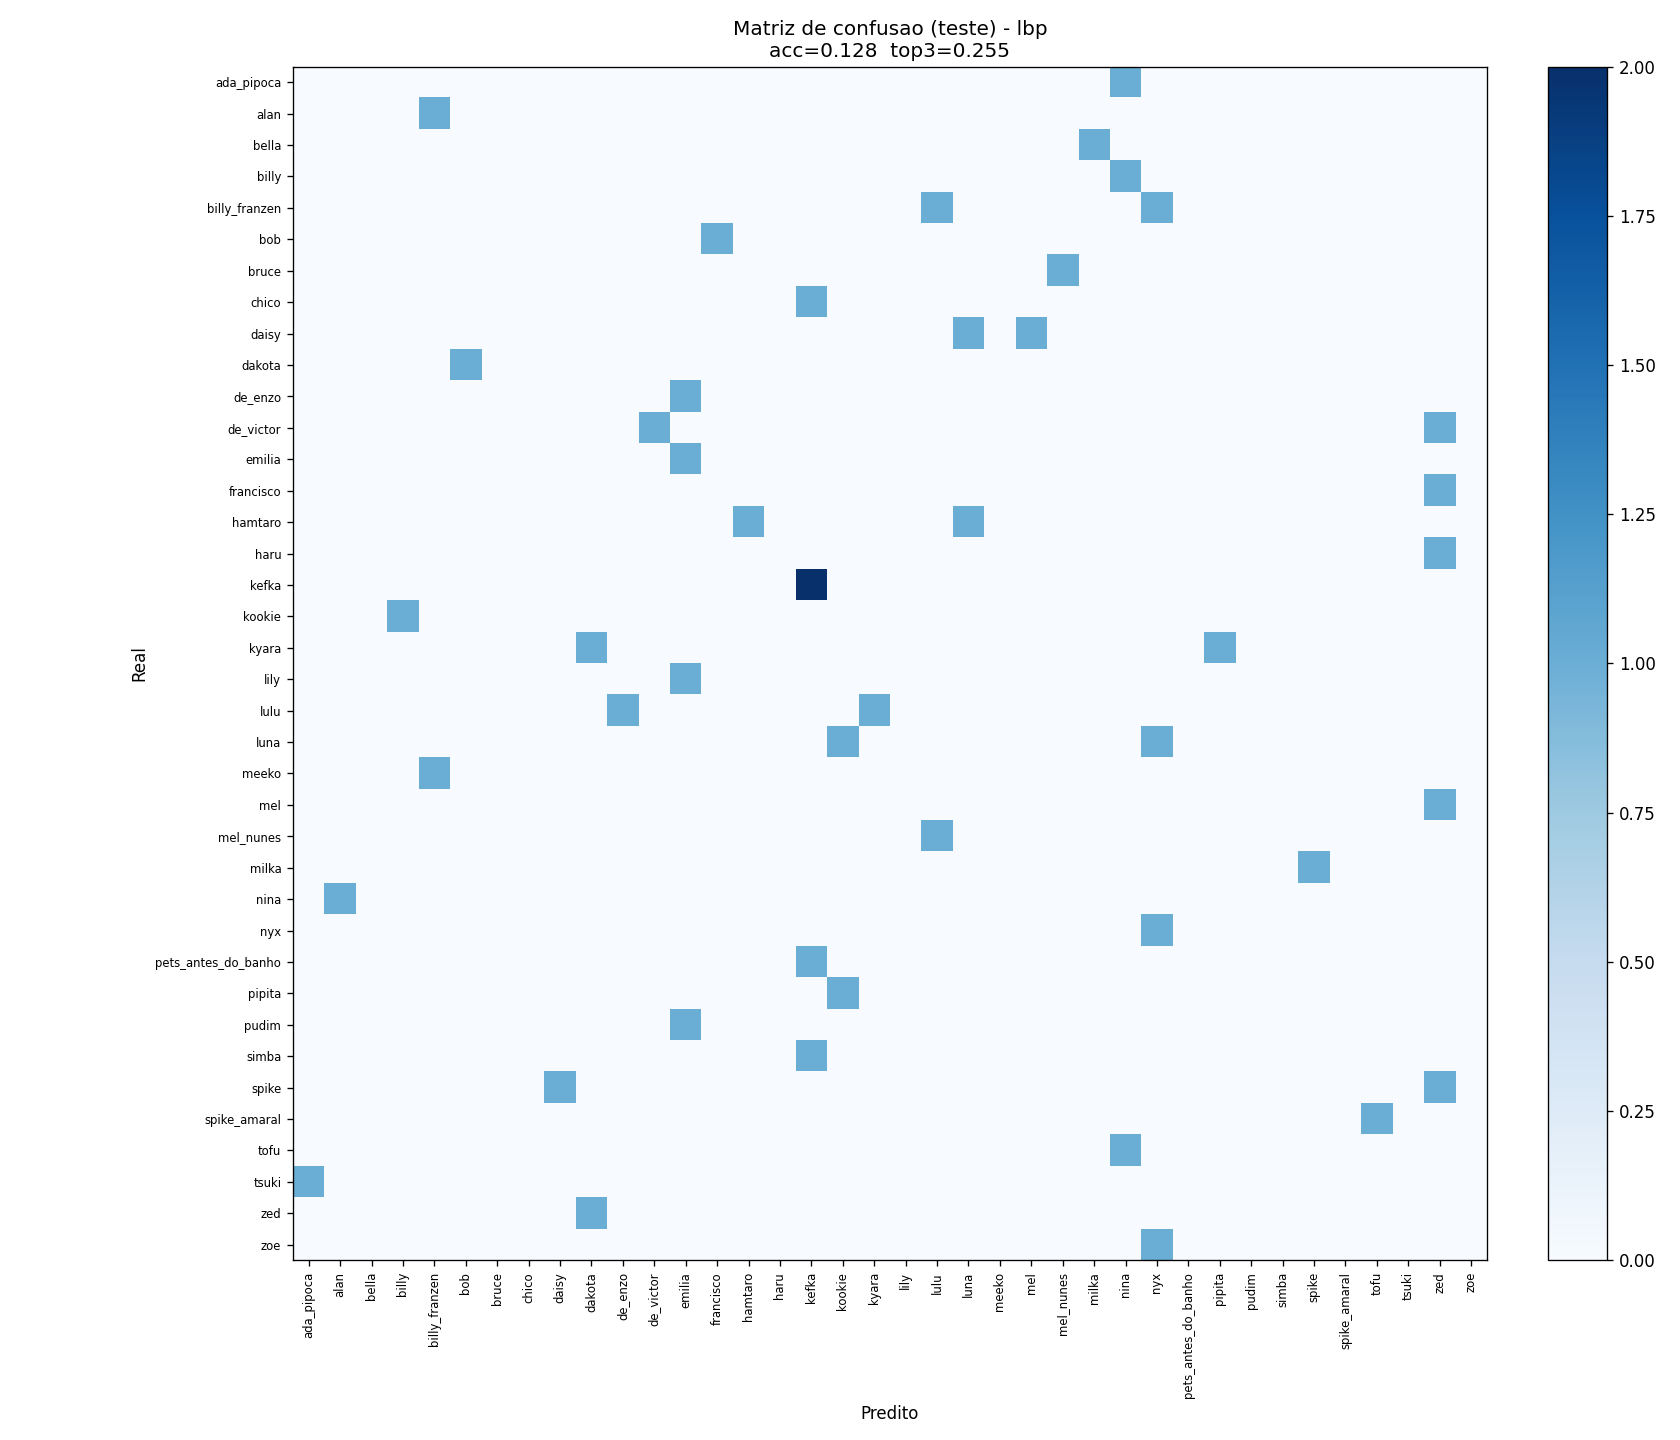
\includegraphics[width=0.75\textwidth]{classificacao_matriz_lbp.png}
    \caption{Matriz de confusão --- LBP isolado.}
\end{figure}

% --- ORB ---
\newpage
\subsection*{3.4 ORB --- keypoints binários}

\textbf{Justificativa da escolha:} ORB foi escolhido especificamente como base para o \textbf{Bag of Visual Words} (seção 6), e não para uso direto. Diferente dos outros 4 descritores, ORB retorna \textbf{número variável de vetores} por imagem (uma lista de $\sim$198 keypoints), o que impede comparação direta por distância euclidiana entre imagens. O BoVW resolve isso agregando os keypoints num histograma de tamanho fixo.

\textbf{Semântica capturada:} pontos visualmente marcantes (cantos, bordas fortes, manchas) descritos por vetores binários invariantes a rotação e escala.

\textbf{Implementação:} \texttt{skimage.feature.ORB(n\_keypoints=200)}. Saída: lista de até 200 keypoints por imagem, cada um com vetor binário de 256 bits. Cobertura: 367/367 imagens com keypoints detectados (média 198 kp/img).

\textbf{Hipótese:}
\begin{itemize}
    \item \textbf{Classificação:} não usado isoladamente (tamanho variável).
    \item \textbf{Busca:} agregado via BoVW. Espera-se desempenho modesto, pois keypoints respondem a ``mesma cena'' mais do que ``mesmo pet'' --- variações de pose e iluminação produzem conjuntos de keypoints muito diferentes para o mesmo animal.
\end{itemize}

\textbf{Resultado observado:} BoVW com K=128 deu P@1 $= 15.5\%$, P@5 $= 8.5\%$ --- pior que HSV puro.

\textbf{Confirmou a hipótese?} Sim. Detalhamento e visualização na seção 6.

% --- GABOR ---
\subsection*{3.5 Banco de Filtros de Gabor --- descritor \textit{não visto em aula}}

\textbf{Justificativa da escolha:} precisávamos de \textbf{um descritor fora do conteúdo de aula} (requisito do enunciado). Optamos por Gabor entre as alternativas (GLCM/Haralick também foi considerado) porque (i) é historicamente um dos descritores mais usados em visão computacional --- foi a base para reconhecimento facial pré-deep learning; (ii) tem \textbf{motivação biológica} (modela células do córtex visual primário V1); (iii) captura textura em \textbf{múltiplas escalas e orientações}, o que LBP não faz; (iv) sua construção (kernel gaussiano modulado, convolução por FFT) usa exatamente as ferramentas vistas na aula de \textbf{restauração} da professora, então é didaticamente coerente com a disciplina.

\textbf{Semântica capturada:} resposta da imagem a um banco de filtros sensíveis a padrões oscilantes (listras) em frequências e orientações variadas. Para cada filtro, guardamos média e desvio padrão da magnitude do output --- resumo estatístico simples mas informativo.

\textbf{Implementação:} \textbf{manual}. Kernel construído pela fórmula clássica (gaussiana 2D $\times$ cosseno/seno, rotacionada por $\theta$); convolução via \textbf{FFT} seguindo o \texttt{filter\_fd} da aula de restauração. 4 frequências $\times$ 4 orientações $\times$ 2 estatísticas = 32 features.

\textbf{Hipótese:}
\begin{itemize}
    \item \textbf{Classificação:} desempenho médio sozinho, melhor que LBP por cobrir múltiplas escalas. Esperamos complementaridade forte com HSV --- cor + textura é o casamento clássico.
    \item \textbf{Busca:} similar --- médio sozinho, bom quando combinado com HSV.
\end{itemize}

\textbf{Resultado observado:} classificação acc $= 19.1\%$, busca P@1 $= 18.0\%$ (segundo melhor isolado, acima de LBP e HOG). \textbf{Combinação HSV+Gabor foi a melhor configuração tanto em classificação (acc $= 34.0\%$, top-3 $= 42.6\%$) quanto em busca (P@1 $= 26.2\%$, P@5 $= 16.7\%$).}

\textbf{Confirmou a hipótese?} Sim, plenamente. As matrizes \texttt{classificacao\_matriz\_gabor.png} (Gabor sozinho) e \texttt{classificacao\_matriz\_hsv\_gabor.png} (combinação) mostram a evolução: Gabor capta diferenças de textura entre pets e a melhoria fica evidente quando combinado com HSV.

\begin{figure}[H]
    \centering
    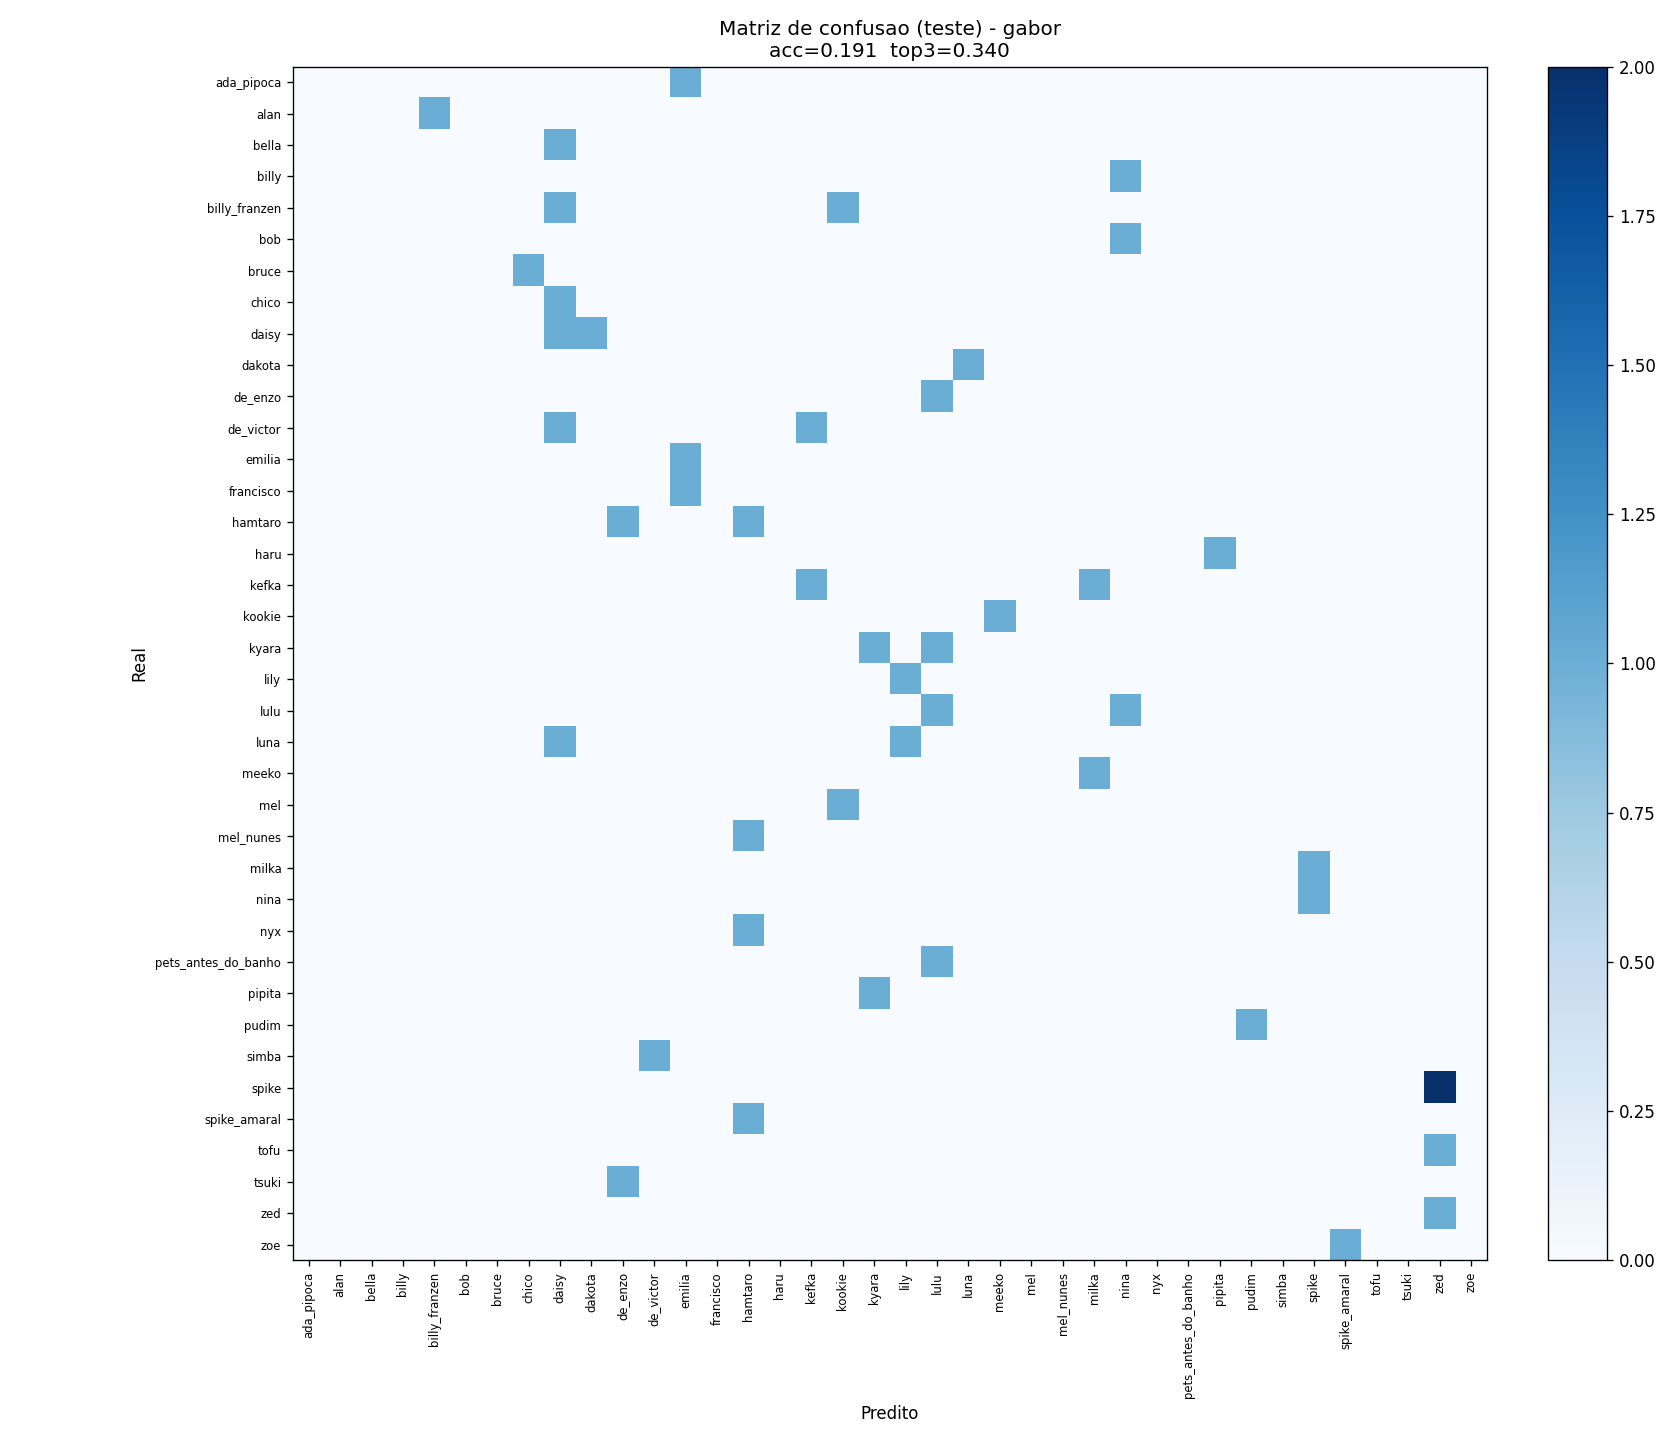
\includegraphics[width=0.75\textwidth]{classificacao_matriz_gabor.png}
    \caption{Matriz de confusão --- Gabor isolado.}
\end{figure}

\newpage
\section*{4. Tarefa de Classificação}

\subsection*{4.1 Metodologia}
\begin{itemize}
    \item \textbf{Filtro de classes:} removidas as 5 classes com 1 imagem $\to$ 38 classes, 362 imagens.
    \item \textbf{Split estratificado 80/10/10} manual (sklearn falha com classes de 3-5 amostras): para cada classe com N imagens, garantimos no mínimo 1 amostra de teste e 1 de validação, sempre preservando $\geq 1$ no treino. Tamanhos finais: \textbf{268 treino / 47 validação / 47 teste}.
    \item \textbf{Padronização:} \texttt{StandardScaler} ajustado apenas no treino.
    \item \textbf{Classificador:} Random Forest com 300 árvores, \texttt{class\_weight='balanced'} e \texttt{random\_state=42}.
    \item \textbf{Combinações:} cada descritor isolado + concatenações com 2, 3 e 4 descritores fixos.
    \item \textbf{Métricas:} acurácia de validação, acurácia de teste e \textbf{acurácia top-3} (a classe correta está entre as 3 mais prováveis).
\end{itemize}

\subsection*{4.2 Resultados}
\begin{table}[H]
\centering
\begin{tabularx}{\textwidth}{X r r r r}
\toprule
\textbf{Combinação} & \textbf{dim} & \textbf{acc val} & \textbf{acc test} & \textbf{top-3} \\
\midrule
hsv                & 96   & 0.255          & 0.298          & \textbf{0.489} \\
hog                & 8100 & 0.085          & 0.128          & 0.191          \\
lbp                & 10   & 0.191          & 0.128          & 0.255          \\
gabor              & 32   & 0.170          & 0.191          & 0.340          \\
hsv+hog            & 8196 & 0.149          & 0.319          & 0.383          \\
hsv+lbp            & 106  & 0.234          & 0.255          & 0.447          \\
\textbf{hsv+gabor} & 128  & \textbf{0.277} & \textbf{0.340} & 0.426          \\
hog+lbp            & 8110 & 0.191          & 0.149          & 0.319          \\
hog+gabor          & 8132 & 0.106          & 0.191          & 0.340          \\
lbp+gabor          & 42   & 0.213          & 0.149          & 0.340          \\
hsv+hog+lbp        & 8206 & 0.234          & 0.106          & 0.319          \\
hsv+hog+lbp+gabor  & 8238 & 0.128          & 0.191          & 0.298          \\
\bottomrule
\end{tabularx}
\caption{Resultados de classificação para cada descritor e combinação.}
\end{table}

Acurácia aleatória esperada $= 1/38 \approx 2.6\%$; estamos consistentemente acima disso.

\subsection*{4.3 Análise}
\begin{itemize}
    \item \textbf{HSV é o descritor mais informativo isoladamente} (acc $= 29.8\%$, top-3 $= 48.9\%$). Confirma a hipótese --- pets têm cores distintivas.
    \item \textbf{HOG é o pior} sozinho (acc $= 12.8\%$). Hipótese confirmada: 8100 features para $\sim$290 amostras de treino é demais --- Random Forest não consegue selecionar splits úteis nessa dimensionalidade.
    \item \textbf{HSV+Gabor é a melhor combinação} (acc val $= 27.7\%$, acc test $= 34.0\%$, top-3 $= 42.6\%$). Isso é coerente com a complementaridade que prevíamos: cor + textura cobrem aspectos diferentes da aparência do pet.
    \item \textbf{Combinações com HOG pioram} os resultados em geral porque os 8100 features do HOG dominam o vetor concatenado mesmo após padronização (problema de dimensionalidade desbalanceada).
    \item \textbf{Top-3 chega a quase 49\%} para HSV sozinho --- o classificador ``quase acerta'' em metade dos casos, errando entre pets visualmente similares.
\end{itemize}

\subsection*{4.4 Limitação metodológica importante}
Com apenas \textbf{47 imagens de teste} distribuídas em 38 classes ($\approx 1.2$ amostras por classe), os valores absolutos têm \textbf{alta variância} --- uma única imagem que dá certo/errado por sorte do split move a acurácia em $\sim 2\%$. Por isso usamos a \textbf{acurácia de validação} como critério oficial para escolher a melhor combinação (\texttt{hsv+gabor}). Para uma estimativa mais robusta seria desejável repetir o split com múltiplas seeds aleatórias e tirar a média $\pm$ desvio padrão, mas isso vai além do escopo pedido pelo enunciado (80/10/10).

\subsection*{4.5 Matrizes de confusão --- melhor combinação}
A figura abaixo mostra a matriz de confusão da combinação \texttt{hsv+gabor} (melhor configuração). Comparada às matrizes individuais (apresentadas nas seções 3.1--3.5), a diagonal aparece mais densa, com acertos múltiplos em \texttt{kefka}, \texttt{kyara}, \texttt{lily}. As confusões remanescentes ocorrem entre pets visualmente parecidos (mesma cor e textura geral) --- o tipo de erro ``natural'' desse problema.

\begin{figure}[H]
    \centering
    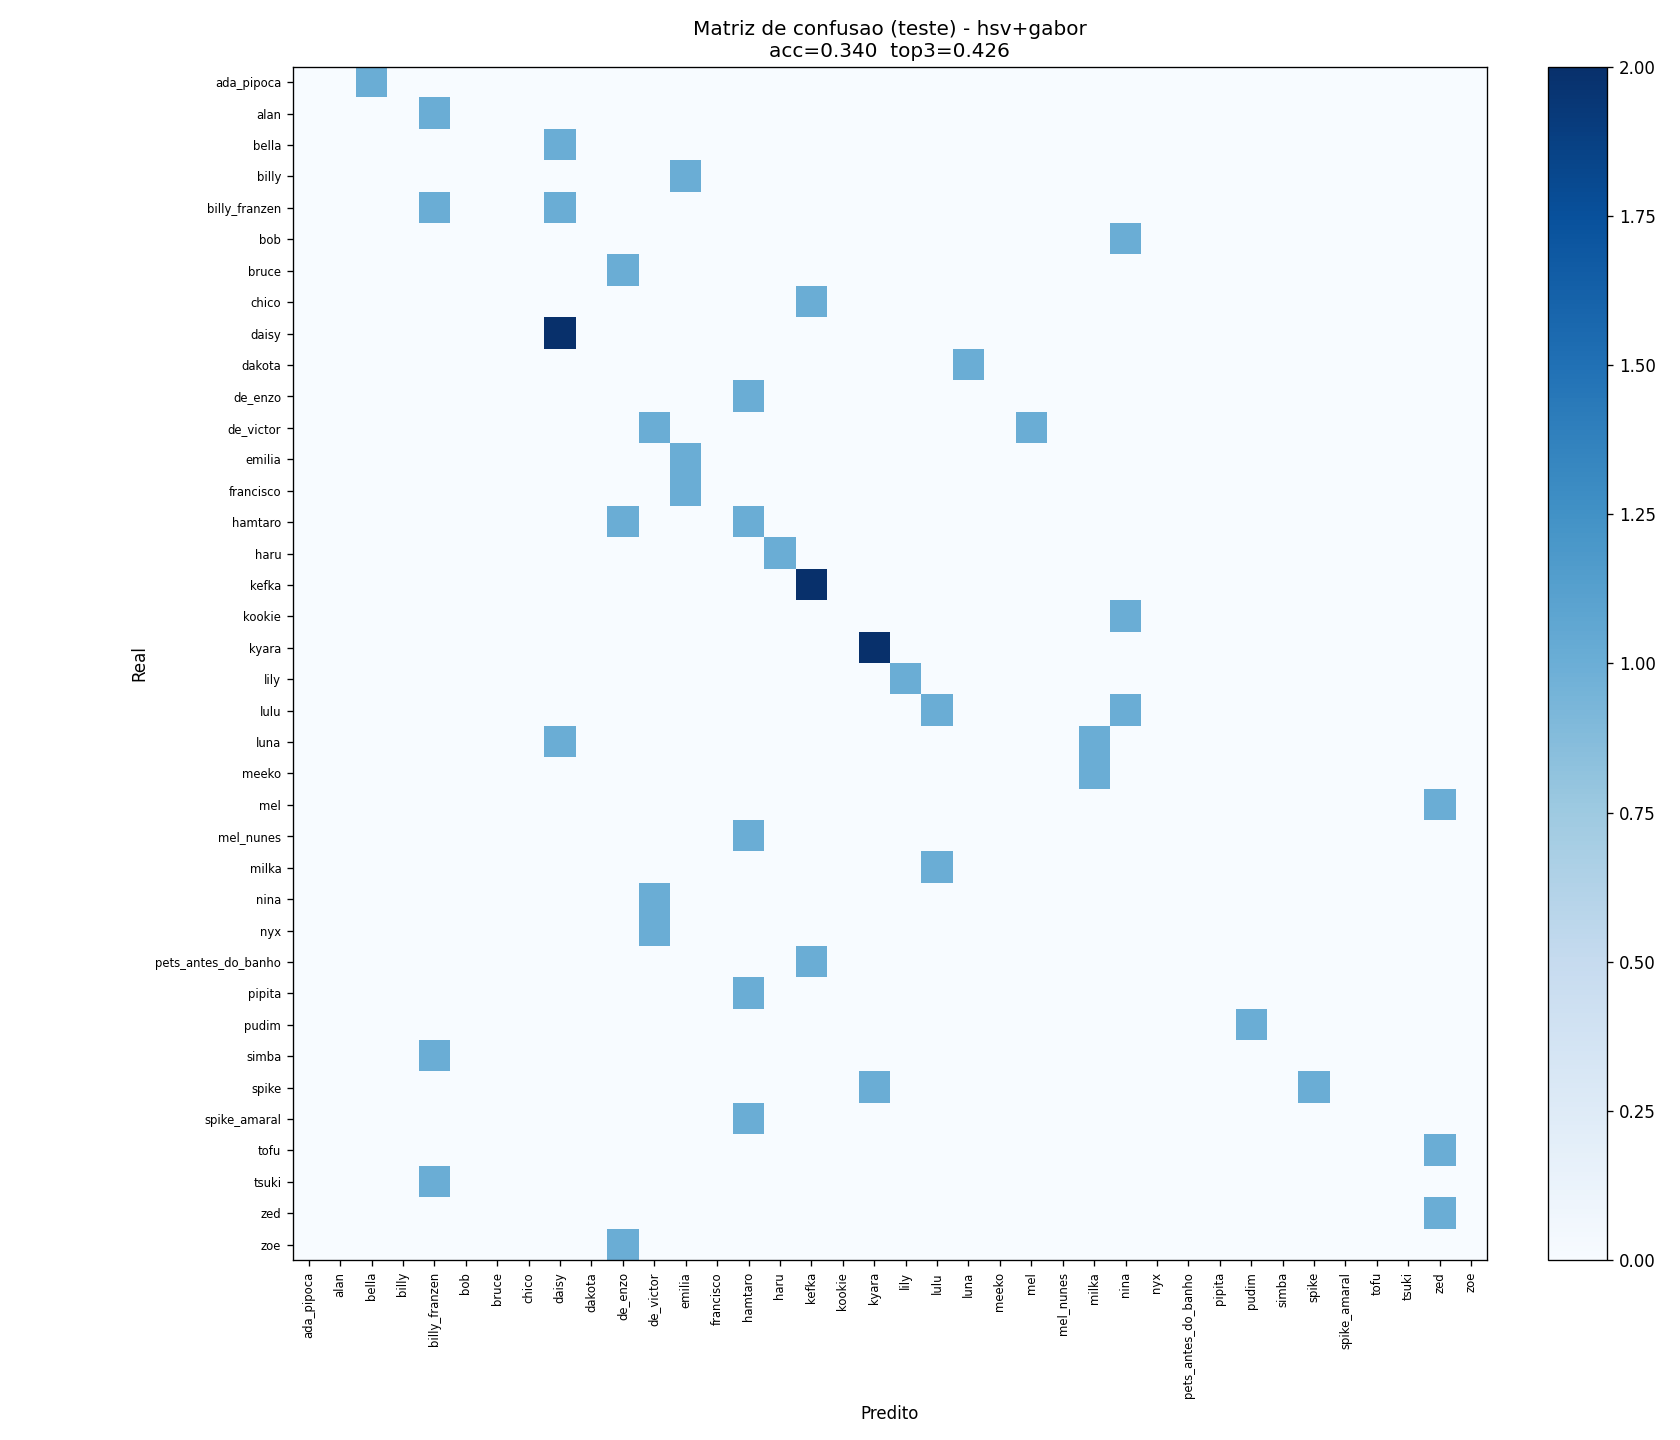
\includegraphics[width=0.85\textwidth]{classificacao_matriz_hsv_gabor.png}
    \caption{Matriz de confusão --- HSV + Gabor (melhor combinação).}
\end{figure}

\newpage
\section*{5. Tarefa de Busca}

\subsection*{5.1 Metodologia}
\begin{itemize}
    \item \textbf{Todas as 367 imagens} participam (busca não exige split treino/teste).
    \item Para cada descritor (ou combinação), aplicamos \textbf{z-score por feature} e concatenamos os blocos antes de calcular \textbf{distância euclidiana par a par}.
    \item Métrica: \textbf{precision@k} --- para cada imagem-consulta (cujas classes têm $\geq 2$ fotos), olhamos os top-$k$ vizinhos mais próximos e medimos quantos são da mesma classe. Reportamos P@1 e P@5.
\end{itemize}

\subsection*{5.2 Resultados}
\begin{table}[H]
\centering
\begin{tabularx}{\textwidth}{X r r r}
\toprule
\textbf{Combinação} & \textbf{dim} & \textbf{P@1} & \textbf{P@5} \\
\midrule
hsv                & 96   & 0.251          & 0.125          \\
hog                & 8100 & 0.094          & 0.057          \\
lbp                & 10   & 0.155          & 0.099          \\
gabor              & 32   & 0.180          & 0.110          \\
hsv+hog            & 8196 & 0.110          & 0.061          \\
hsv+lbp            & 106  & 0.273          & 0.143          \\
\textbf{hsv+gabor} & 128  & \textbf{0.262} & \textbf{0.167} \\
hsv+hog+lbp        & 8206 & 0.110          & 0.060          \\
hsv+hog+lbp+gabor  & 8238 & 0.113          & 0.061          \\
\bottomrule
\end{tabularx}
\caption{Precisão da busca para cada descritor e combinação.}
\end{table}

\subsection*{5.3 Análise}
\begin{itemize}
    \item \textbf{HSV+Gabor vence novamente} (P@1 $= 26.2\%$, P@5 $= 16.7\%$). Mesma combinação que ganhou na classificação --- sugere que cor + textura é um par genuinamente complementar para essa tarefa.
    \item \textbf{HOG aparece consistentemente como ruído} na busca: sozinho dá P@1 $= 9.4\%$, e em qualquer combinação que contenha HOG a métrica despenca. Isso confirma a hipótese de que a dimensionalidade do HOG (8100) domina a distância euclidiana mesmo após z-score por feature.
    \item \textbf{LBP sozinho} dá P@1 $= 15.5\%$, mais que o esperado para um descritor de só 10 features --- textura local é informativa para a base.
    \item \textbf{Gabor sozinho} dá P@1 $= 18.0\%$, acima de LBP, sugerindo que capturar múltiplas escalas/orientações compensa.
\end{itemize}

\subsection*{5.4 Características interessantes nos rankings}
Na figura \texttt{busca\_top5\_hsv\_gabor.png}, observamos:
\begin{itemize}
    \item Para a consulta \texttt{lily} (pomerâniana branca, peluda): top vizinhos contêm dois acertos (\texttt{lily}) e três falsos-positivos que são também \textbf{pets brancos e peludos} (\texttt{spike\_amaral}, \texttt{bruce}). O sistema está acertando o conceito visual (``pet branco fofo''), apenas errando o pet exato.
    \item Para \texttt{bella} (pet caramelo): nenhum acerto no top-5, mas todos os vizinhos são pets pequenos castanho-claros (\texttt{de\_enzo}, \texttt{lulu}, \texttt{luna}). De novo, similaridade visual capturada corretamente.
    \item Para \texttt{haru} (gata preta): top-5 são quase todos pets escuros (\texttt{zed}, \texttt{spike}) --- captura a cor predominante.
\end{itemize}

Esses padrões mostram que o descritor está fazendo o \textbf{trabalho dele}: encontrar fotos visualmente parecidas. Os ``erros'' são erros de identidade do pet, não de similaridade visual --- e isso é o melhor que se pode esperar de descritores que não sabem o que é ``individual'' daquele animal.

\begin{figure}[H]
    \centering
    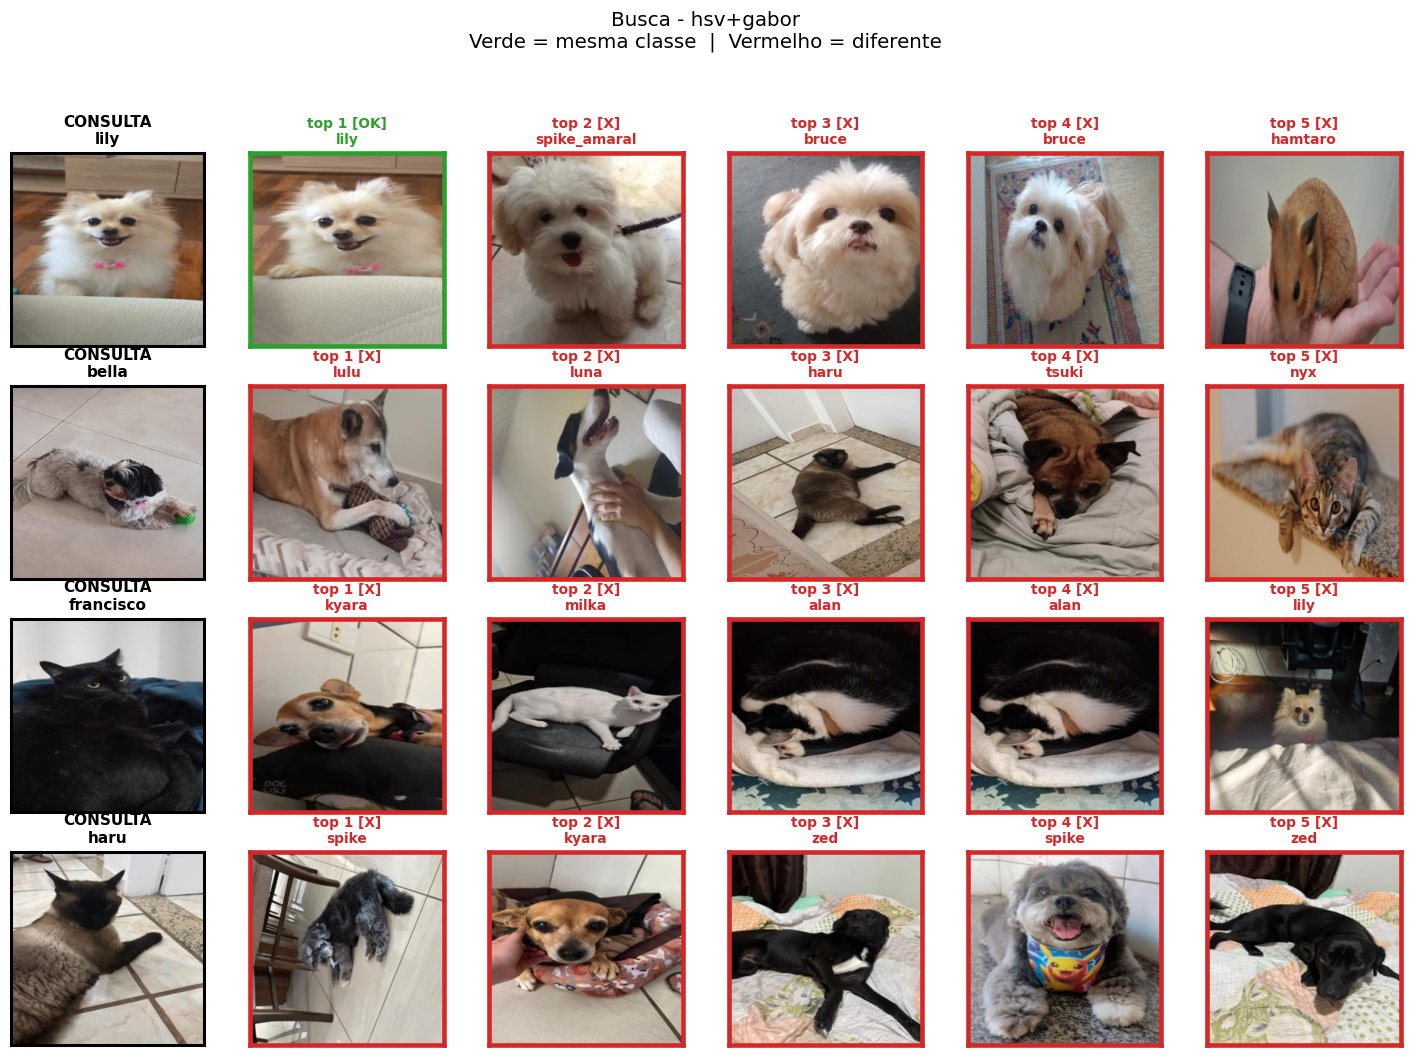
\includegraphics[width=\textwidth]{busca_top5_hsv_gabor.png}
    \caption{Top-5 vizinhos para consultas representativas --- HSV+Gabor.}
\end{figure}

\newpage
\section*{6. Bag of Visual Words (BoVW)}

\subsection*{6.1 Construção}
\begin{itemize}
    \item \textbf{Descritores brutos:} 367 imagens $\times$ $\sim$198 keypoints $=$ \textbf{72.833 vetores ORB} de dimensão 256 (binários).
    \item \textbf{Subamostragem:} 30.000 descritores aleatórios para o KMeans.
    \item \textbf{Vocabulário visual:} \textbf{K=128 palavras} obtidas por \texttt{MiniBatchKMeans}.
    \item \textbf{Histograma por imagem:} cada keypoint é atribuído à palavra mais próxima; o histograma resultante (128 bins) é normalizado L1.
    \item \textbf{Busca:} distância euclidiana entre histogramas.
\end{itemize}

\subsection*{6.2 Resultado}
\textbf{BoVW (K=128): P@1 $= 0.155$ --- P@5 $= 0.085$.} Pior que HSV puro e muito pior que HSV+Gabor.

\subsection*{6.3 Análise}
\begin{itemize}
    \item BoVW captura \textbf{estatística de keypoints} --- quais regiões ``marcantes'' aparecem na imagem. Pets em poses, iluminações e ângulos diferentes produzem keypoints muito diferentes, o que dilui o sinal de identidade.
    \item \textbf{Não tem cor:} ORB trabalha em escala de cinza. Isso explica boa parte da queda em relação a HSV.
    \item Em bases com muitas fotos por classe (centenas), BoVW costuma se dar bem; com $\sim$3--20 fotos por classe, há poucas evidências para o KMeans agrupar palavras ``típicas'' de cada pet.
\end{itemize}

\subsection*{6.4 Visualização (UMAP e t-SNE da BoVW)}
As figuras a seguir mostram os 367 histogramas de visual words projetados em 2D. As 10 classes com mais imagens estão coloridas, as demais em cinza claro.

\begin{figure}[H]
    \centering
    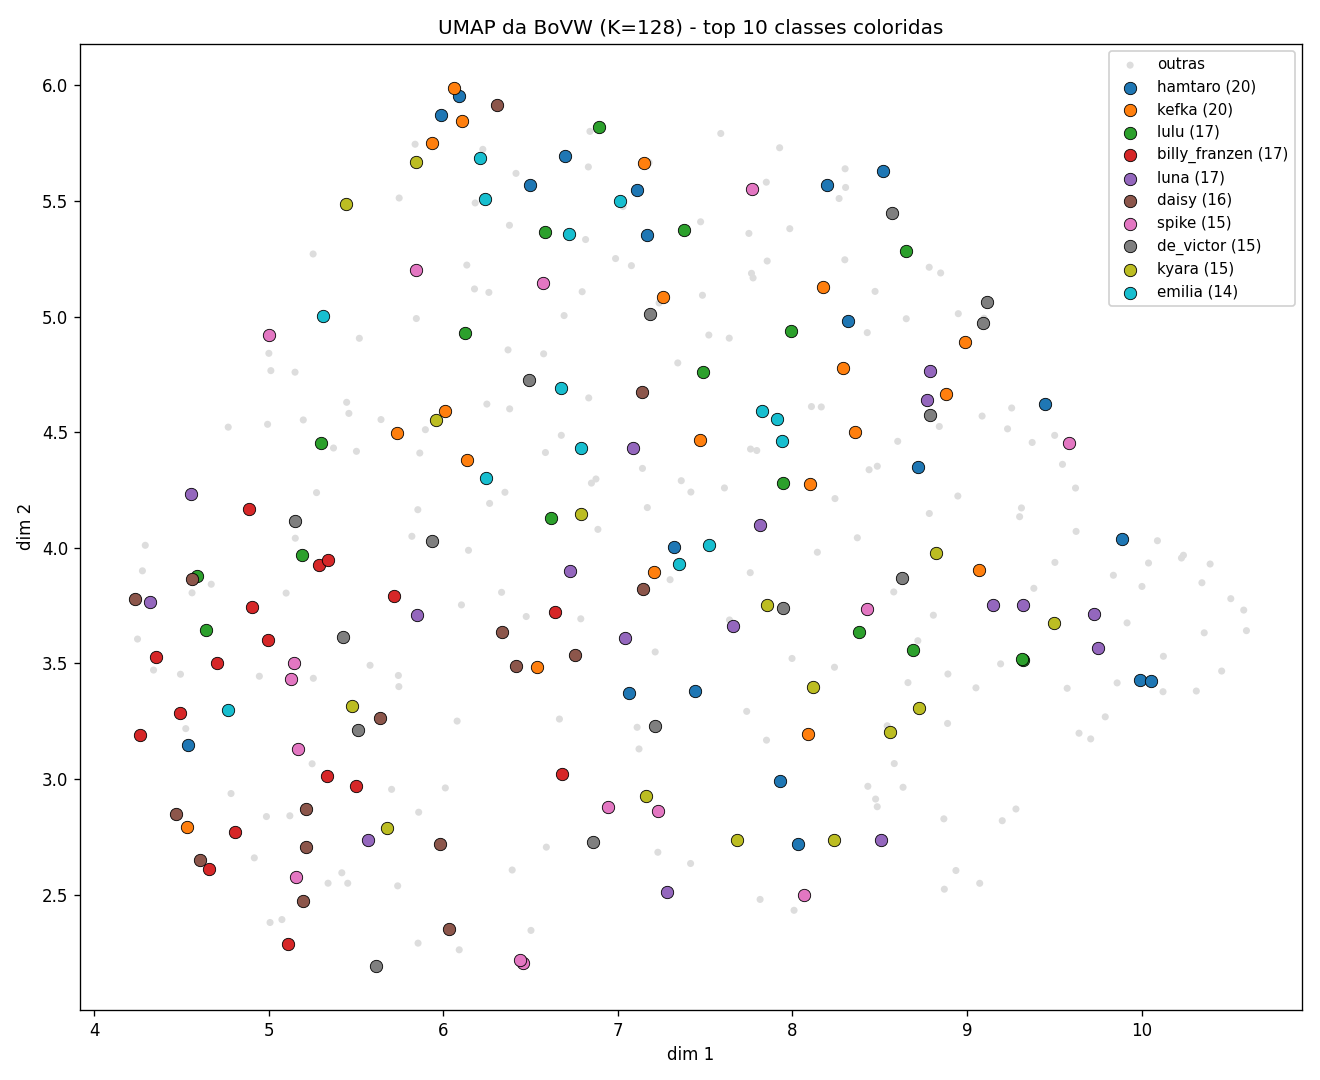
\includegraphics[width=0.85\textwidth]{visualizacao_bovw_umap.png}
    \caption{Projeção UMAP dos histogramas BoVW.}
\end{figure}

\begin{figure}[H]
    \centering
    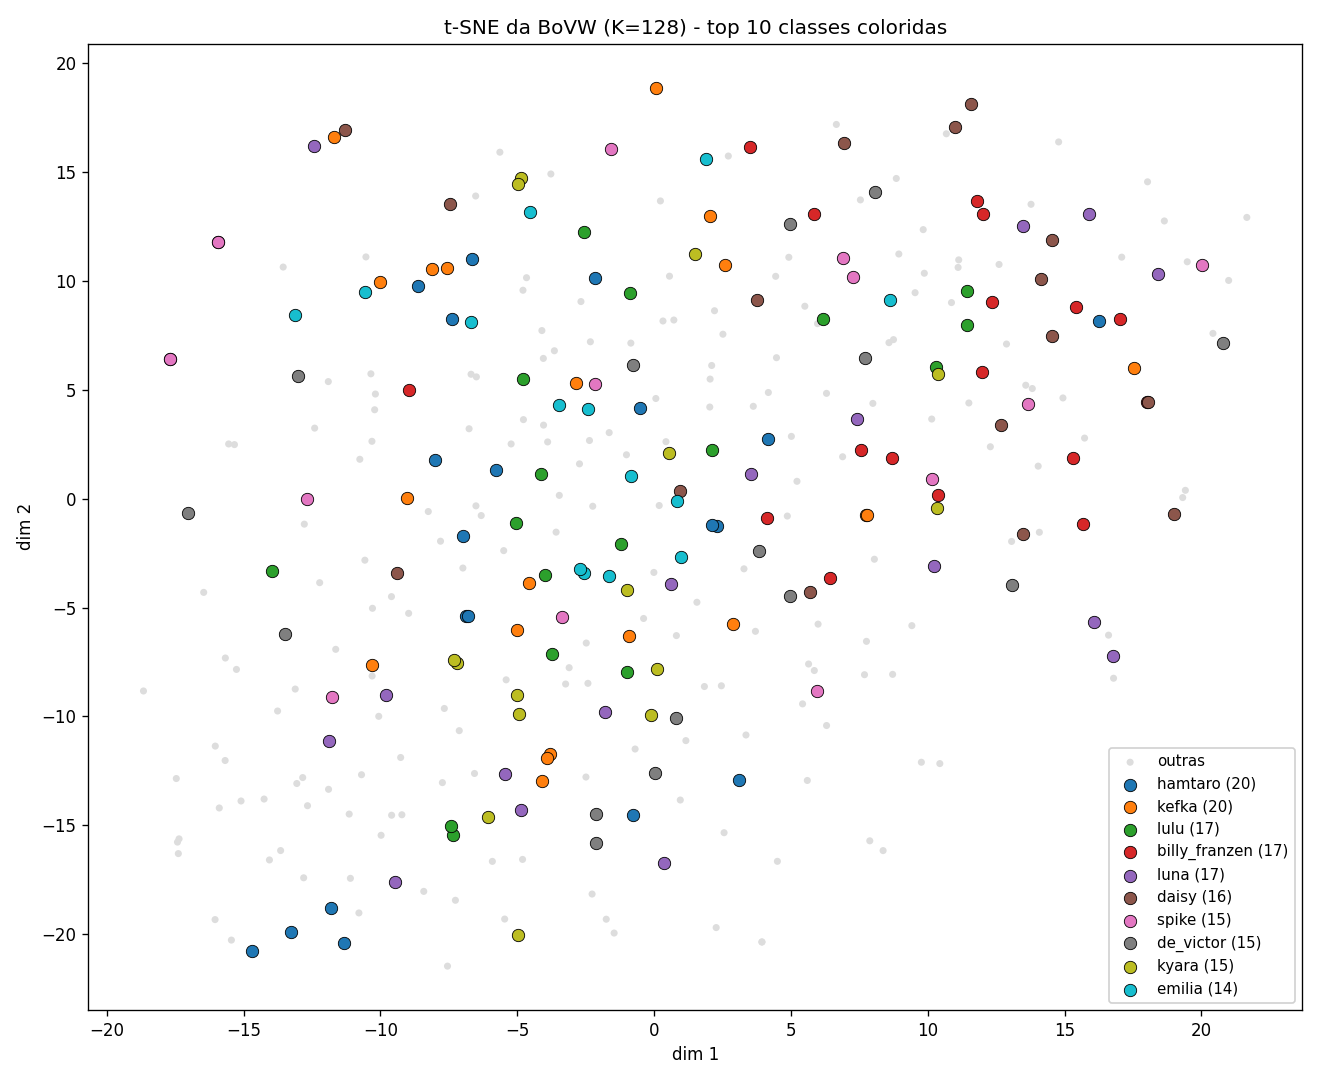
\includegraphics[width=0.85\textwidth]{visualizacao_bovw_tsne.png}
    \caption{Projeção t-SNE dos histogramas BoVW.}
\end{figure}

\textbf{Observação principal:} pontos de uma mesma classe (mesma cor) estão \textbf{espalhados por todo o plano}, sem formar clusters identificáveis.

\textbf{Hipóteses para essa distribuição:}
\begin{enumerate}
    \item \textbf{Variabilidade intra-classe alta:} cada pet aparece em fotos com iluminação, fundo e pose muito diferentes, gerando histogramas BoVW bem distintos para a mesma classe.
    \item \textbf{Vocabulário visual genérico:} com K=128 palavras treinadas em todos os pets juntos, as palavras tendem a representar \textbf{estruturas comuns} (olhos, focinho, cantos de mobília) que aparecem em vários pets --- não discriminam identidade individual.
    \item \textbf{ORB não captura cor:} o que diferencia pets visualmente (cor do pelo) é justamente o que o BoVW por ORB ignora --- então as classes acabam misturadas no espaço.
\end{enumerate}

A coerência das duas projeções (UMAP e t-SNE mostrando o mesmo padrão de mistura) reforça que essa não é uma falha de visualização --- é uma propriedade do \textbf{descritor BoVW por ORB} para essa base específica.

\newpage
\section*{7. Conclusões}
\begin{itemize}
    \item \textbf{Melhor combinação para ambas as tarefas:} \textbf{HSV + Gabor} (cor + textura estatística). Para classificação: acc test $= 34.0\%$ (top-3 $= 42.6\%$). Para busca: P@1 $= 26.2\%$, P@5 $= 16.7\%$.
    \item \textbf{HSV sozinho} já é um baseline forte (acc $29.8\%$, top-3 $48.9\%$) e confirma a importância da cor para identificar pets.
    \item \textbf{HOG é prejudicial} quando combinado por causa da sua altíssima dimensionalidade (8100), que domina a distância euclidiana mesmo após padronização. Para uso futuro, valeria reduzir HOG com PCA antes de combinar.
    \item \textbf{BoVW por ORB foi o pior} para essa base --- keypoints binários em escala de cinza não capturam o suficiente da identidade do pet, e a alta variabilidade intra-classe dilui o histograma.
    \item \textbf{Top-3 $\approx 49\%$} mostra que o sistema ``quase acerta'' em metade dos casos --- os erros são tipicamente entre pets visualmente parecidos.
    \item \textbf{Limitação fundamental:} a base é pequena e desbalanceada para 38 classes. Os números absolutos têm alta variância por causa do tamanho do conjunto de teste (47 imagens, $\sim 1.2$ por classe).
\end{itemize}

\section*{8. Bibliotecas usadas}
\begin{table}[H]
\centering
\begin{tabularx}{\textwidth}{l l X}
\toprule
\textbf{Biblioteca} & \textbf{Uso} & \textbf{Justificativa} \\
\midrule
\texttt{numpy}, \texttt{matplotlib}, \texttt{imageio.v3} & utilitários & mesmo stack da professora \\
\texttt{skimage.feature.\{hog, LBP, ORB\}} & descritores 2, 3, 4 & usado em \texttt{aulas/segmentacao/cod2.py} \\
\texttt{skimage.color.rgb2hsv} & descritor 1 & usado em \texttt{aulas/cores/Aula17-Clean.ipynb} \\
\texttt{sklearn.\{ensemble, preprocessing, metrics, cluster, manifold\}} & classificador, padronização, BoVW, t-SNE & enunciado autoriza \\
\texttt{umap-learn} & visualização BoVW & enunciado cita ``UMAP ou t-SNE'' \\
\bottomrule
\end{tabularx}
\end{table}

O descritor \textbf{Gabor} foi implementado manualmente (kernel + convolução por FFT), seguindo a fórmula clássica e o estilo da função \texttt{filter\_fd} da aula de restauração da professora.

\section*{9. Arquivos entregues}
\begin{itemize}
    \item \texttt{codigos/descritores.py} --- 5 extratores
    \item \texttt{codigos/extrai\_features.py} --- pipeline de extração
    \item \texttt{codigos/classificacao.py} --- pipeline de classificação
    \item \texttt{codigos/busca.py} --- pipeline de busca
    \item \texttt{codigos/bovw.py} --- pipeline BoVW
    \item \texttt{codigos/visualizacao.py} --- UMAP + t-SNE
    \item \texttt{features/*.npy}, \texttt{features/orb.pkl} --- vetores extraídos
    \item \texttt{resultados/*.png}, \texttt{resultados/*.txt} --- figuras e tabelas
    \item \texttt{relatorio3.tex} (este arquivo)
\end{itemize}

\end{document}
